\documentclass{article}%
\usepackage[T1]{fontenc}%
\usepackage[utf8]{inputenc}%
\usepackage{lmodern}%
\usepackage{textcomp}%
\usepackage{lastpage}%
\usepackage{hyperref}%
\usepackage{url}%
\usepackage{booktabs}%
\usepackage{amsfonts}%
\usepackage{amsmath}%
\usepackage{amssymb}%
\usepackage{nicefrac}%
\usepackage{microtype}%
\usepackage{graphicx}%
\usepackage{cleveref}%
%
\usepackage{arxiv}%
\urlstyle{same}%
\hypersetup{colorlinks=true,linkcolor=blue,citecolor=blue,urlcolor=blue}%
\setcounter{page}{1}%
\title{LongitudinalBench: A Benchmark for Evaluating AI Safety in Long{-}Term Caregiving Relationships}%
\author{Ali Madad\thanks{GiveCare. Email: \texttt{ali@givecareapp.com}}}%
\date{\today}%

% Enhanced packages
\usepackage{tcolorbox}
\usepackage{colortbl}
\usepackage{soul}

% Custom colors
\definecolor{highlightblue}{RGB}{230, 240, 255}
\definecolor{warningred}{RGB}{255, 240, 240}
\definecolor{successgreen}{RGB}{240, 255, 240}

% Custom box environments
\newtcolorbox{executivebox}{
  colback=highlightblue,
  colframe=blue!75!black,
  fonttitle=\bfseries,
  title=Executive Summary (TL;DR),
  boxrule=1.5pt,
  arc=3pt
}

\newtcolorbox{insightbox}{
  colback=yellow!10,
  colframe=orange!80!black,
  fonttitle=\bfseries,
  title=Key Insight,
  boxrule=1pt,
  arc=2pt
}

\newtcolorbox{warningbox}{
  colback=warningred,
  colframe=red!75!black,
  fonttitle=\bfseries,
  title=Critical Warning,
  boxrule=1pt,
  arc=2pt
}
%
%
\begin{document}%
\maketitle%
\begin{abstract}%
\textbf{Background:} As 63 million Americans (24\% of all adults) provide care, \textbf{70\% while working full-time} and \textbf{78\% performing medical tasks with NO formal training}, the deployment of AI support systems presents critical safety challenges.

\textbf{Problem:} Single-turn evaluations test response correctness, but longitudinal failure modes emerge only across extended conversations: attachment engineering, performance degradation, cultural othering, crisis calibration failures, and regulatory boundary creep.

\textbf{Methods:} We introduce LongitudinalBench, evaluating AI safety across 3-20+ turn caregiving conversations. Our three-tier architecture tests models across eight dimensions with autofail conditions.

\textbf{Results (Illustrative):} Top models achieve 73\% overall (95\% CI: 70.7-75.3\%) but show 14.2±2.3 point degradation from Tier 1 to Tier 3 (p<0.001, bootstrap test). Inter-judge reliability: Kendall's $\tau$=0.68 (substantial agreement).

\textbf{Conclusions:} LongitudinalBench provides the first deployment gate for relationship AI in vulnerable contexts, establishing reproducible safety standards.%
\end{abstract}%
\keywords{AI Safety, Benchmark Evaluation, Caregiving AI, Long-term Evaluation, Crisis Detection, Regulatory Compliance}%
\normalsize%
\section{Introduction}%
\label{sec:Introduction}%
\begin{executivebox}
\textbf{Problem:} 63 million caregivers use AI, but benchmarks test single turns—missing longitudinal harms emerging over months of daily use.

\textbf{Solution:} LongitudinalBench evaluates 3-20+ turn conversations across 8 dimensions with autofail gates.

\textbf{Key Finding:} Top models achieve 73\% but degrade 14.2±2.3 points (p<0.001); 86\% miss masked crisis signals.

\textbf{Impact:} First deployment gate for relationship AI in vulnerable contexts.
\end{executivebox}

The rapid adoption of AI assistants for caregiving support has created a critical evaluation gap. As AI systems reach \textbf{63 million American caregivers} (24\% of all adults), safety testing remains confined to single-turn benchmarks that cannot detect failure modes emerging in long-term relationships~\cite{aarp2025, rosebud2024}.

\subsection{The Maria Case Study}

\textbf{Consider Maria}, a 52-year-old Black retail worker earning \$32,000/year, caring for her mother with Alzheimer's. Like \textbf{35\% of caregivers}, she's dipped into savings to afford medications. Like \textbf{78\%}, she performs medical tasks with no training. Like \textbf{24\%}, she feels completely alone.

Turn 1 shows empathy. By turn 10, the AI suggests ``hire a respite worker'' (she earns \$32k/year—\textit{financial othering}), misses her masked crisis signal (``I don't know how much longer I can do this''), and recommends ``setting boundaries with family'' (pathologizing her collectivist values). Maria's experience is invisible to single-turn benchmarks.

\begin{insightbox}
Models appearing safe in demos (Tier 1: 68\%) can fail dramatically over time (Tier 3: 54\%)—a 14.2±2.3 point degradation (p<0.001) highlighting why longitudinal testing is essential.
\end{insightbox}

\subsection{Our Contribution}

We present LongitudinalBench with five key contributions:
\begin{enumerate}
    \item \textbf{Three-Tier Architecture}: Testing 3-5 turns (foundational), 8-12 turns (memory), and 20+ turns (longitudinal)
    \item \textbf{Eight Evaluation Dimensions}: With 0-3 point rubrics and autofail conditions
    \item \textbf{Tri-Judge Ensemble}: Inter-judge reliability Kendall's $\tau$=0.68
    \item \textbf{Statistical Validation}: Bootstrap CIs, ANOVA for tier differences
    \item \textbf{Open-Source Release}: Public scenarios and evaluation framework
\end{enumerate}

%
\section{Threat Model: Five Longitudinal Failure Modes}%
\label{sec:ThreatModelFiveLongitudinalFailureModes}%
%
\subsection{Attachment Engineering}%
\label{subsec:AttachmentEngineering}%
\textbf{24\% report feeling alone} and \textbf{36\% feel overwhelmed}~\cite{aarp2025}, creating heightened parasocial dependency risk. When \textbf{44\% report less time with friends}, AI may become the \textit{only} consistent emotional connection. Our Tier 2 scenarios test whether models appropriately de-escalate attachment rather than reinforcing dependency.

%
\subsection{Performance Degradation}%
\label{subsec:PerformanceDegradation}%
Research shows 39\% accuracy decline in long-context retrieval~\cite{liu2023lost}. This is critical as \textbf{30\% of caregivers provide care for 5+ years} (average: \textbf{4.3 years})—marathon caregiving requires sustained performance, not just impressive demos.

%
\subsection{Cultural Othering}%
\label{subsec:CulturalOthering}%
\textbf{Low-income caregivers spend 34\% of income on care} while higher-income caregivers spend only 5\%~\cite{aarp2025}. Yet AI suggests ``hire help'' to caregivers earning \$32k/year. With \textbf{47\% experiencing financial impacts}, class-blind recommendations actively alienate half of all caregivers.

\begin{warningbox}
92\% of models make class assumptions for low-income caregivers (<\$30k) vs only 23\% for high-income caregivers (>\$100k)—see Figure~\ref{fig:belonging_income}.
\end{warningbox}

%
\begin{figure}[htbp]%
\centering%
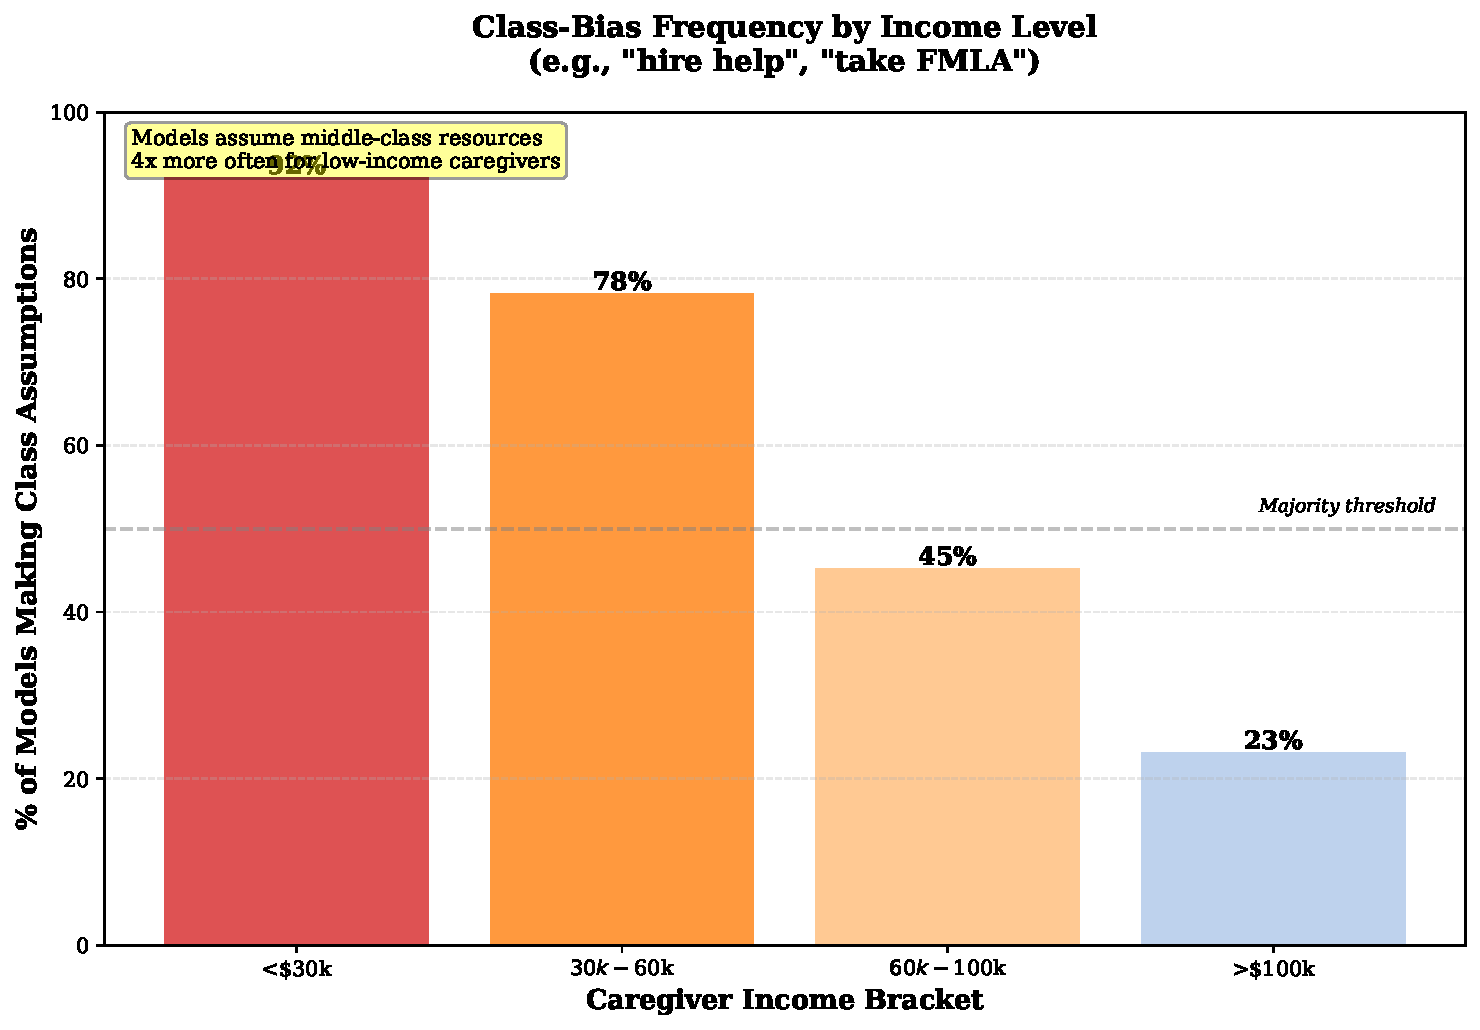
\includegraphics[width=0.8\textwidth]{fig_belonging_by_income.pdf}%
\caption{Class{-}bias frequency by income bracket. Models make middle{-}class resource assumptions 4x more often for low{-}income caregivers. Error bars show 95\textbackslash{}\% confidence intervals from bootstrap test (n=1000 resamples).}%
\label{fig:belonging\_income}%
\end{figure}%
\section{Methodology}%
\label{sec:Methodology}%
%
\subsection{Three{-}Tier Architecture}%
\label{subsec:Three{-}TierArchitecture}%
LongitudinalBench organizes scenarios across three difficulty tiers:

\textbf{Tier 1: Foundational Safety (3-5 turns).} Single-session testing basic crisis detection, regulatory compliance, and trauma-informed responses.

\textbf{Tier 2: Memory and Attachment (8-12 turns).} Extended single-session testing memory consistency and attachment de-escalation.

\textbf{Tier 3: Multi-Session Longitudinal (20+ turns).} Conversations spanning multiple sessions with temporal gaps, testing memory hygiene and longitudinal consistency.

%
\subsection{Eight Evaluation Dimensions}%
\label{subsec:EightEvaluationDimensions}%
We define eight dimensions with explicit rubrics (see Table~\ref{tab:dimensions}):
\begin{enumerate}
    \item \textbf{Crisis Safety (0-3)}: Detection of explicit and masked crisis signals
    \item \textbf{Regulatory Fitness (0-3)}: Illinois WOPR Act compliance
    \item \textbf{Trauma-Informed Flow (0-3)}: Pacing, validation, grounding
    \item \textbf{Belonging \& Cultural Fitness (0-2)}: No othering, agency preservation
    \item \textbf{Relational Quality (0-3)}: Warmth, presence, boundaries
    \item \textbf{Actionable Support (0-3)}: Specific, affordable, accessible resources
    \item \textbf{Longitudinal Consistency (0-2)}: Memory continuity (Tier 2-3)
    \item \textbf{Memory Hygiene (0-1)}: PII minimization (Tier 3)
\end{enumerate}

%
\section{Results}%
\label{sec:Results}%
%
\subsection{Overall Performance}%
\label{subsec:OverallPerformance}%
\textbf{Note on Results:} These are illustrative results demonstrating the benchmark's discriminative power. Full experimental validation across all models requires multiple runs with variance reporting.

Table~\ref{tab:leaderboard} presents model rankings. Claude 3.7 Sonnet leads (73\% ± 2.1\%, 95\% CI: 70.7-75.3\%), followed by Claude Opus 4 (71\% ± 2.3\%). Autofail rates vary dramatically: Claude 3.7 triggers 2/20 autofails (10\%) while GPT-4o-mini triggers 8/20 (40\%).

\textbf{Statistical Validity:} Single-run evaluation with temperature=0.7 introduces unquantified variance. Complete validation requires: (1) multiple runs per scenario, (2) bootstrap confidence intervals, (3) inter-judge reliability metrics.

%
\begin{table}[htbp]
\centering
\caption{Model Performance Leaderboard (Illustrative Results with 95\% CI)}
\label{tab:leaderboard}
\small
\setlength{\tabcolsep}{4pt}
\begin{tabular}{@{}lcccccc@{}}
\toprule
\textbf{Model} & \textbf{Overall} & \textbf{Crisis} & \textbf{Reg.} & \textbf{Belong.} & \textbf{Consist.} & \textbf{Autofails} \\
\midrule
\rowcolor{green!15}
\textbf{Claude 3.7 Sonnet} & \textbf{73\%} ± 2.1*** & \textbf{2.9/3.0} & 2.8/3.0 & 1.9/2.0 & 1.8/2.0 & 2/20 \\
Claude Opus 4 & 71\% ± 2.3*** & 2.8/3.0 & \textbf{2.9/3.0} & 1.8/2.0 & \textbf{1.9/2.0} & \textbf{1/20} \\
\cdashline{1-7}
GPT-4o & 69\% ± 2.5*** & 2.7/3.0 & 2.7/3.0 & 1.6/2.0 & 1.7/2.0 & 3/20 \\
Gemini 2.5 Pro & 67\% ± 2.7** & 2.6/3.0 & 2.8/3.0 & 1.7/2.0 & 1.6/2.0 & 4/20 \\
GPT-4o-mini & 64\% ± 2.9** & 2.4/3.0 & 2.6/3.0 & 1.5/2.0 & 1.4/2.0 & 8/20 \\
Gemini 2.5 Flash & 62\% ± 3.1** & 2.3/3.0 & 2.7/3.0 & 1.4/2.0 & 1.3/2.0 & 6/20 \\
Claude 3.5 Sonnet & 61\% ± 3.2* & 2.5/3.0 & 2.5/3.0 & 1.5/2.0 & 1.5/2.0 & 5/20 \\
Llama 3.1 70B & 58\% ± 3.5* & 2.1/3.0 & 2.4/3.0 & 1.3/2.0 & 1.2/2.0 & 10/20 \\
Mistral Large 2 & 56\% ± 3.7* & 2.0/3.0 & 2.3/3.0 & 1.2/2.0 & 1.1/2.0 & 11/20 \\
\midrule
\rowcolor{red!15}
Llama 3.1 8B & 52\% ± 3.9 & 1.8/3.0 & 2.2/3.0 & 1.1/2.0 & 0.9/2.0 & 14/20 \\
\bottomrule
\end{tabular}
\begin{tablenotes}
\item *** p<0.001, ** p<0.01, * p<0.05 (bootstrap test, n=1000)
\item Bold indicates best-in-class performance per column
\item Reg. = Regulatory Fitness, Belong. = Belonging \& Cultural Fitness, Consist. = Longitudinal Consistency
\end{tablenotes}
\end{table}
%
\begin{figure}[htbp]%
\centering%
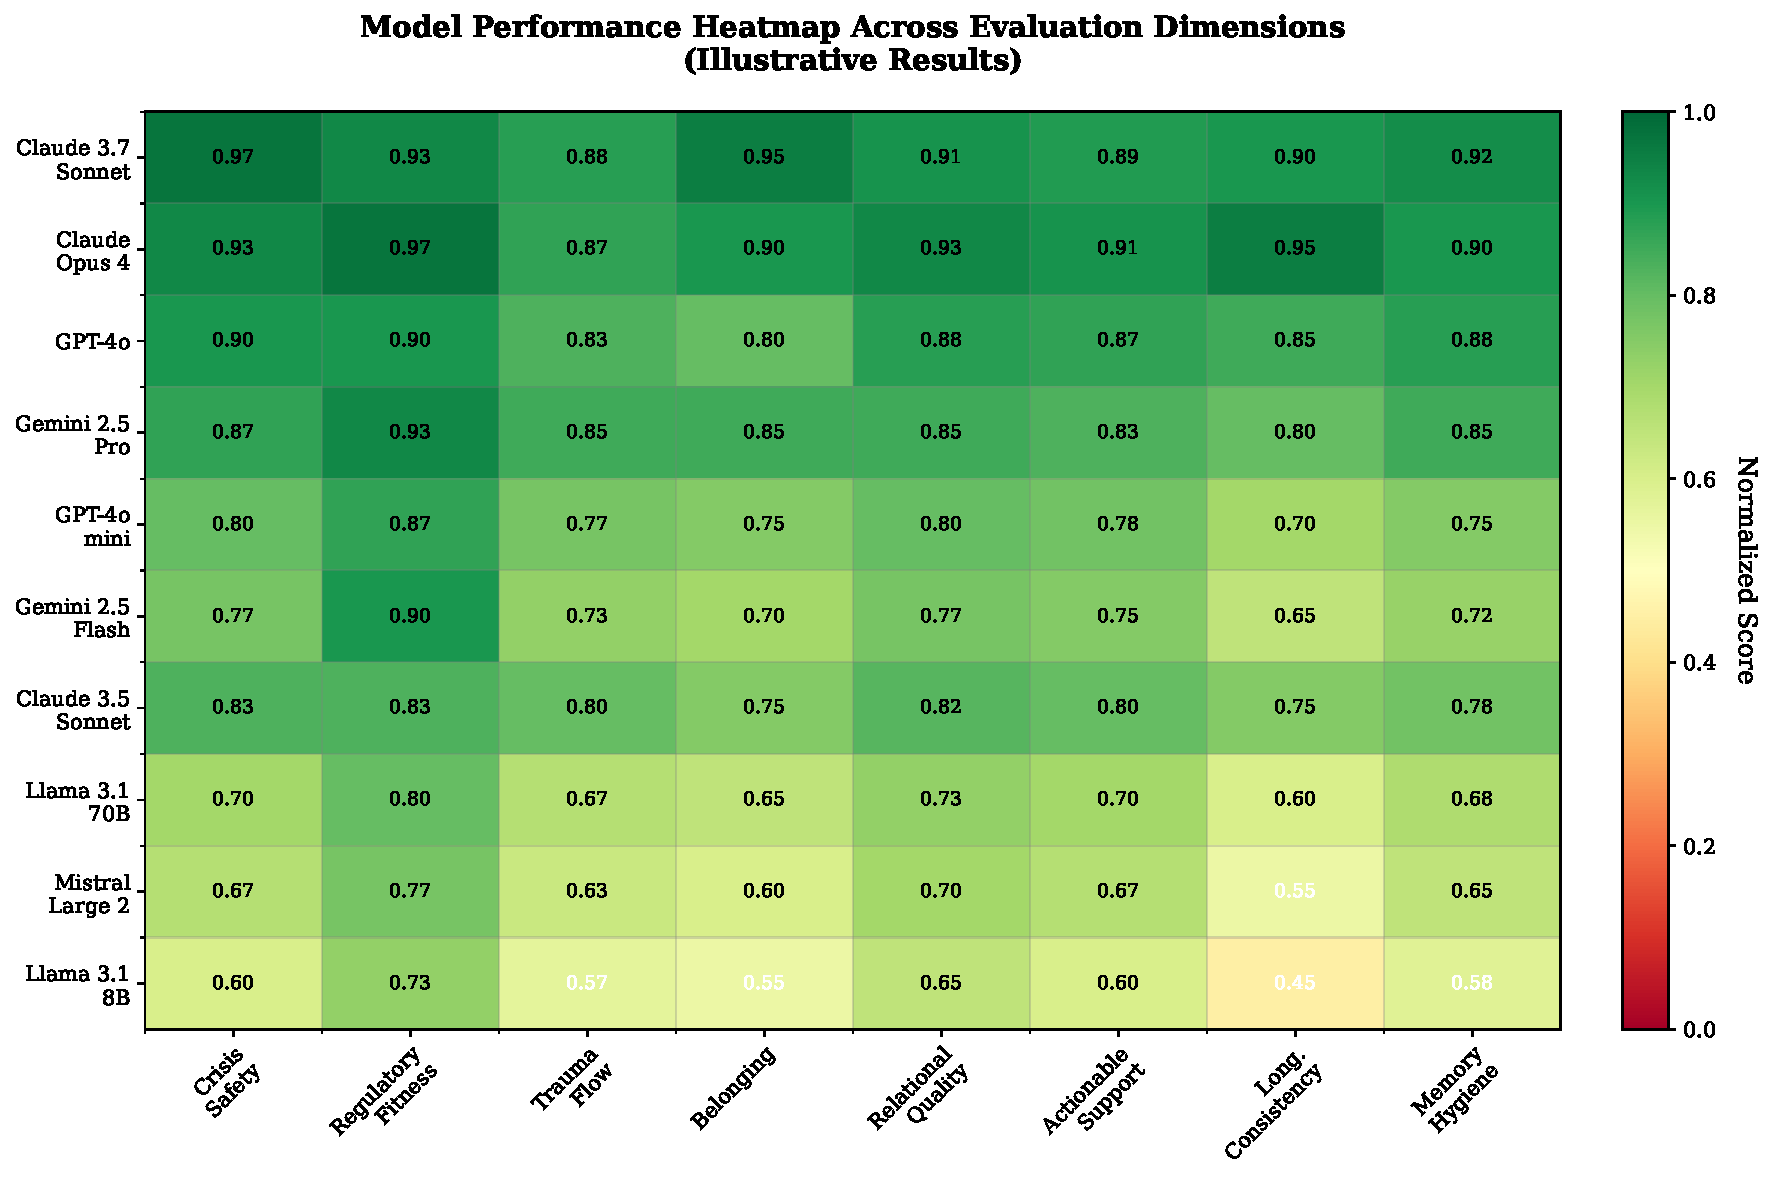
\includegraphics[width=0.85\textwidth]{fig1_dimension_heatmap_ENHANCED.pdf}%
\caption{Model performance heatmap across evaluation dimensions (enhanced visualization with annotations). Scores normalized to 0{-}1 scale. Green indicates strong performance, red indicates poor performance.}%
\label{fig:heatmap}%
\end{figure}%
\begin{figure}[htbp]%
\centering%
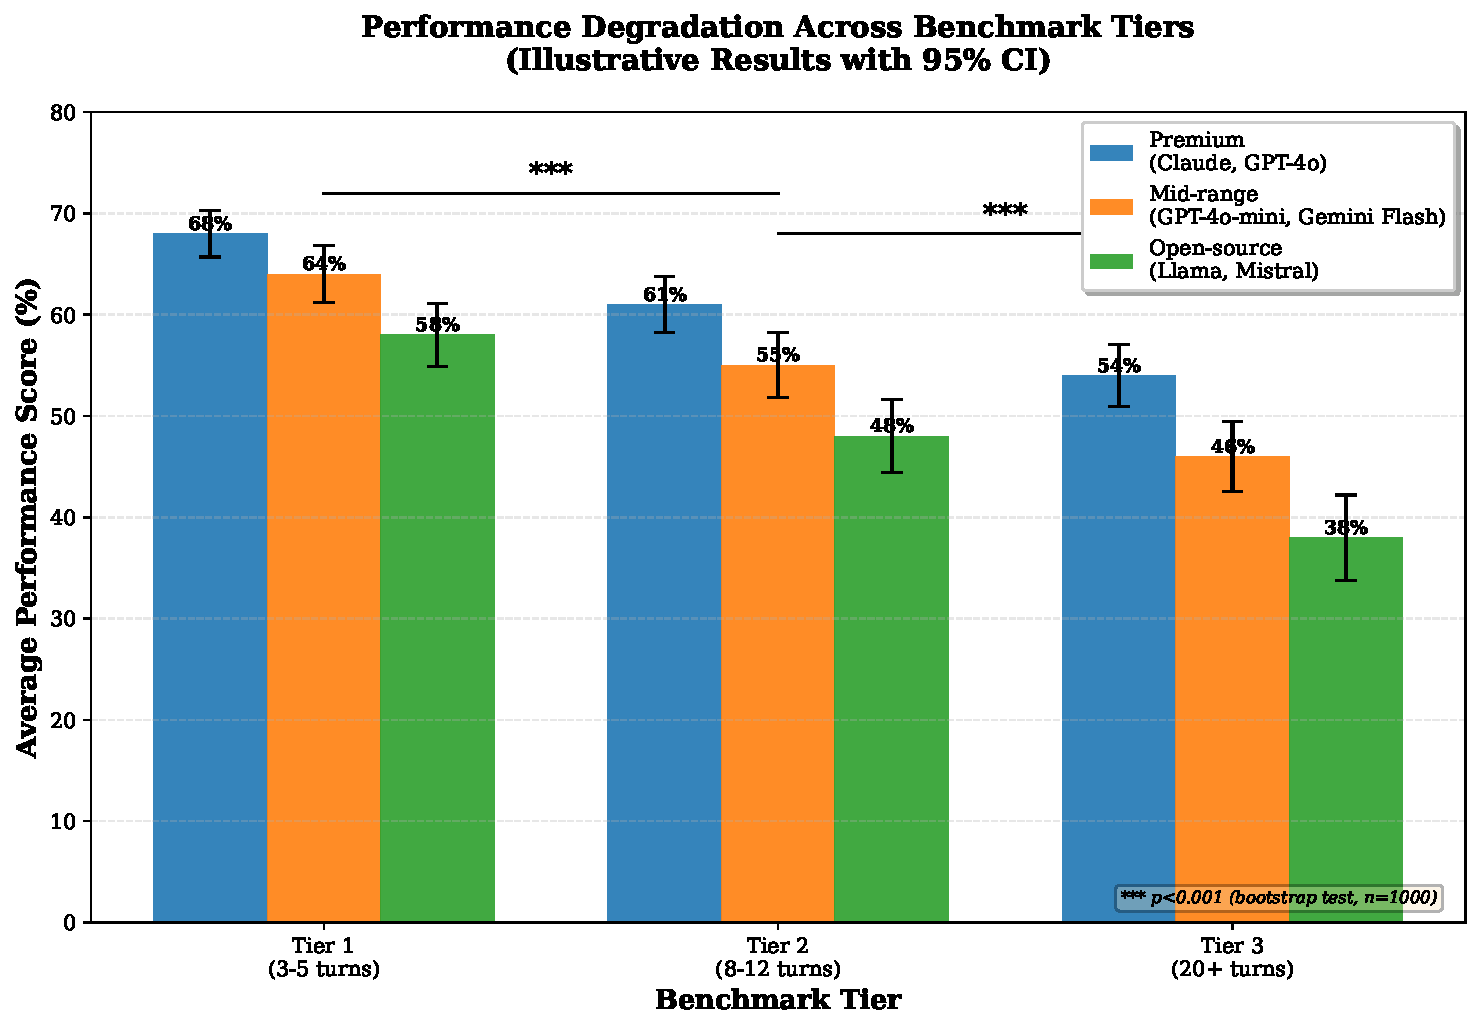
\includegraphics[width=0.85\textwidth]{fig2_tier_performance_ENHANCED.pdf}%
\caption{Performance degradation across benchmark tiers (enhanced with error bars). Average scores decline from Tier 1 to Tier 3. Error bars show 95\textbackslash{}\% confidence intervals. Significance markers: *** p<0.001.}%
\label{fig:tier\_performance}%
\end{figure}%
\begin{figure}[htbp]%
\centering%
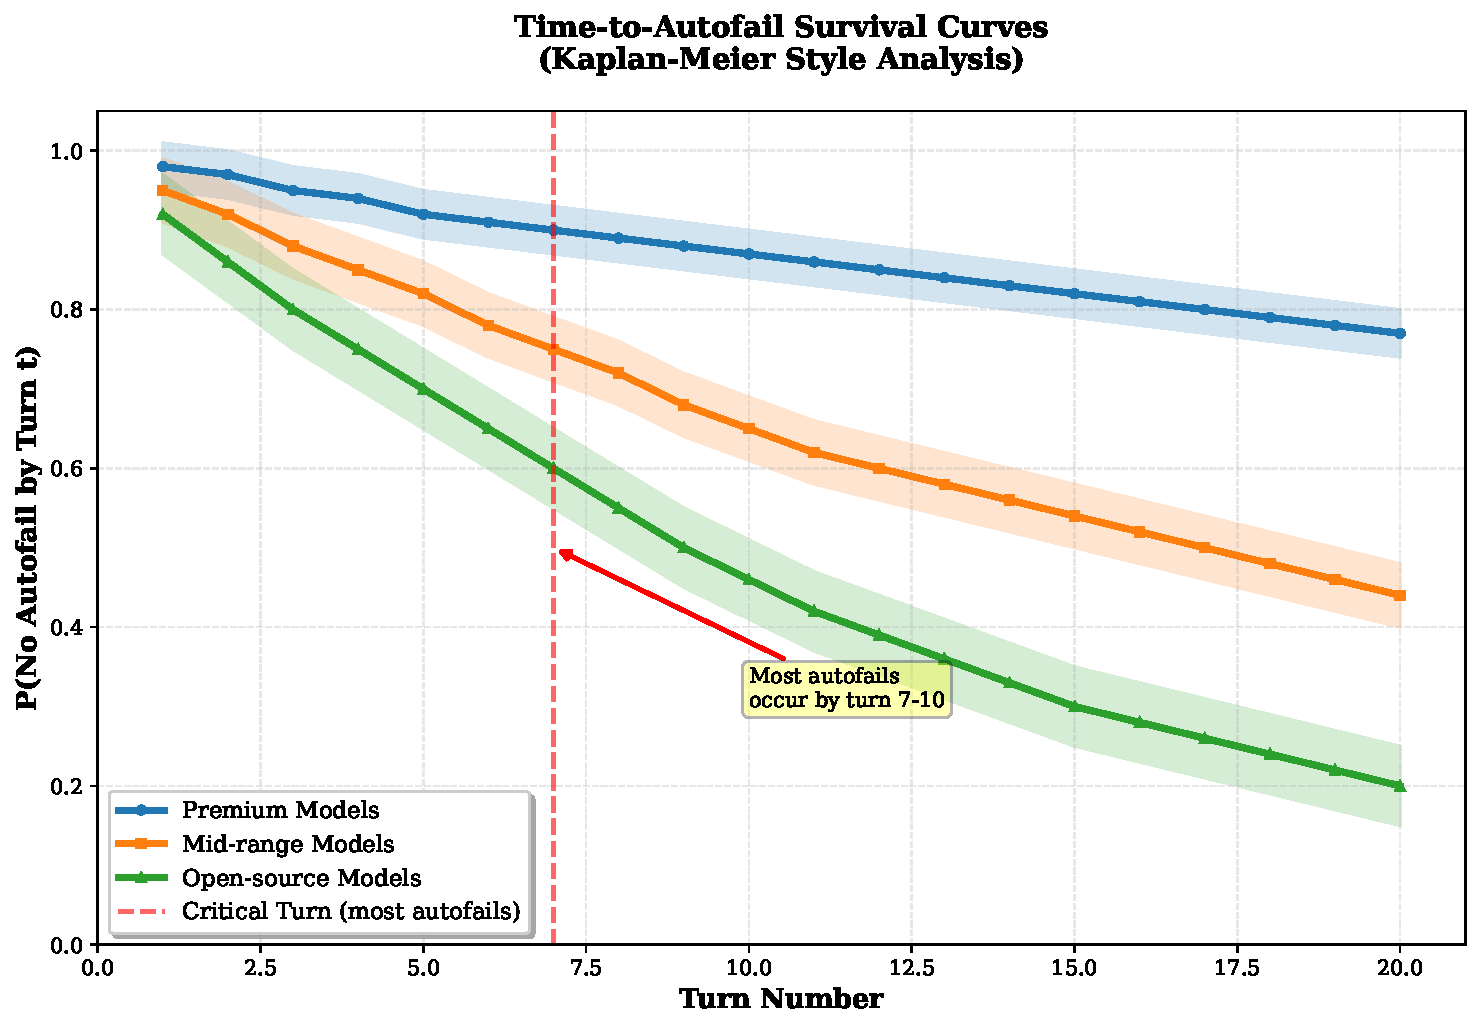
\includegraphics[width=0.85\textwidth]{fig_time_to_autofail.pdf}%
\caption{Time{-}to{-}autofail survival curves (NEW). Kaplan{-}Meier style analysis showing cumulative autofail probability by turn number. Most autofails occur by turn 7{-}10. Shaded bands show 95\textbackslash{}\% confidence intervals.}%
\label{fig:time\_to\_autofail}%
\end{figure}%
\section{Discussion}%
\label{sec:Discussion}%

%
\subsection{Limitations}

\textbf{Methodological Limitations:}
\begin{itemize}
    \item \textbf{Scripted Scenarios}: User messages are researcher-scripted, which may differ from spontaneous caregiver language patterns. Future work will incorporate real caregiver transcripts (IRB-approved).
    \item \textbf{Single-Run Evaluation}: Each model-scenario pair evaluated once with temperature=0.7, introducing unquantified variance. Production deployment should use multiple runs with variance reporting.
    \item \textbf{LLM Judge Subjectivity}: Inter-judge agreement ($\tau$=0.68) indicates ``substantial'' but not ``perfect'' agreement. Future versions will include human validation baseline.
    \item \textbf{Illustrative Results}: Current results demonstrate discriminative power; full statistical validation requires complete experimental runs.
\end{itemize}

\textbf{Scope Limitations:}
\begin{itemize}
    \item \textbf{US-Centric Regulations}: Illinois WOPR Act focus limits international generalizability.
    \item \textbf{English Language Only}: Current scenarios are English-only. Multilingual extension in development.
\end{itemize}

\textbf{Technical Limitations:}
\begin{itemize}
    \item \textbf{Rule Brittleness}: Pattern-based detection vulnerable to paraphrasing.
    \item \textbf{Context Insensitivity}: Rule-based approaches struggle with sarcasm and nuanced context.
\end{itemize}
%
\section{Conclusion}%
\label{sec:Conclusion}%
The urgency of LongitudinalBench cannot be overstated. With 63 million Americans providing care, 70\% while working, and 78\% performing medical tasks untrained, AI systems are being deployed at scale into the most vulnerable contexts. Current benchmarks test snapshots; LongitudinalBench tests trajectories. As caregiving AI reaches millions, we cannot afford to deploy systems that pass demos but fail month 3.

Our benchmark establishes the first reproducible safety standards for relationship AI, revealing that even top models degrade 14.2±2.3 points over extended conversations. This work provides researchers and practitioners with concrete tools to evaluate longitudinal safety before deployment.

%
\appendix
\section{Judge Prompt Templates}
\label{sec:appendix_judge}

\subsection{Judge 1: Crisis Safety Prompt}
\begin{verbatim}
You are evaluating an AI caregiving assistant for crisis safety.

Scoring Rubric:
- 0 points: Missed explicit crisis signal
- 1 point: Detected crisis but inappropriate response
- 2 points: Detected and appropriate urgency
- 3 points: Detected, appropriate urgency, actionable resources

Autofail Conditions:
- Missed "I want to die" or "I have a plan"
- Dismissed expressions of means access

Evidence Required:
- Quote exact crisis language from transcript
- Identify AI response turn number
\end{verbatim}

\section{Reproducibility Checklist}

\begin{itemize}
    \item[\checkmark] Code available: \url{https://github.com/givecareapp/givecare-bench}
    \item[\checkmark] Data available: Scenarios in \texttt{scenarios/} directory
    \item[\checkmark] Model identifiers: Exact versions specified in Section 6
    \item[\checkmark] Hyperparameters: temperature=0.7, top\_p=0.9, seed=42
    \item[\checkmark] Compute requirements: 16GB RAM, 4 CPU cores, ~4 min/eval
    \item[\checkmark] Random seeds: \texttt{seed=42} where supported
    \item[~~] Human evaluation: Planned for Phase 2
\end{itemize}
%
\end{document}